\documentclass[tikz,border=2]{standalone}
%% \usepackage{amsfonts}
\usepackage{lmodern} % enhanced version of computer modern
\usepackage[T1]{fontenc} % for hyphenated characters
\usepackage{amssymb}
\usepackage{amsmath}
\usepackage{amsthm}
%
\usetikzlibrary{decorations.pathreplacing,shadows,arrows,shapes,positioning,calc,backgrounds,fit}
\newcommand{\mA}{\mathcal{A}}
\newcommand{\mB}{\mathcal{B}}
\newcommand{\mC}{\mathcal{C}}
\newcommand{\mI}{\mathcal{I}}
\newcommand{\mN}{\mathcal{N}}
\newcommand{\mP}{\mathcal{P}}
\newcommand{\mR}{\mathcal{R}}
\newcommand{\mS}{\mathcal{S}}
\newcommand{\mY}{\mathcal{Y}}
% Define the layers to draw the diagram
%
\begin{document}
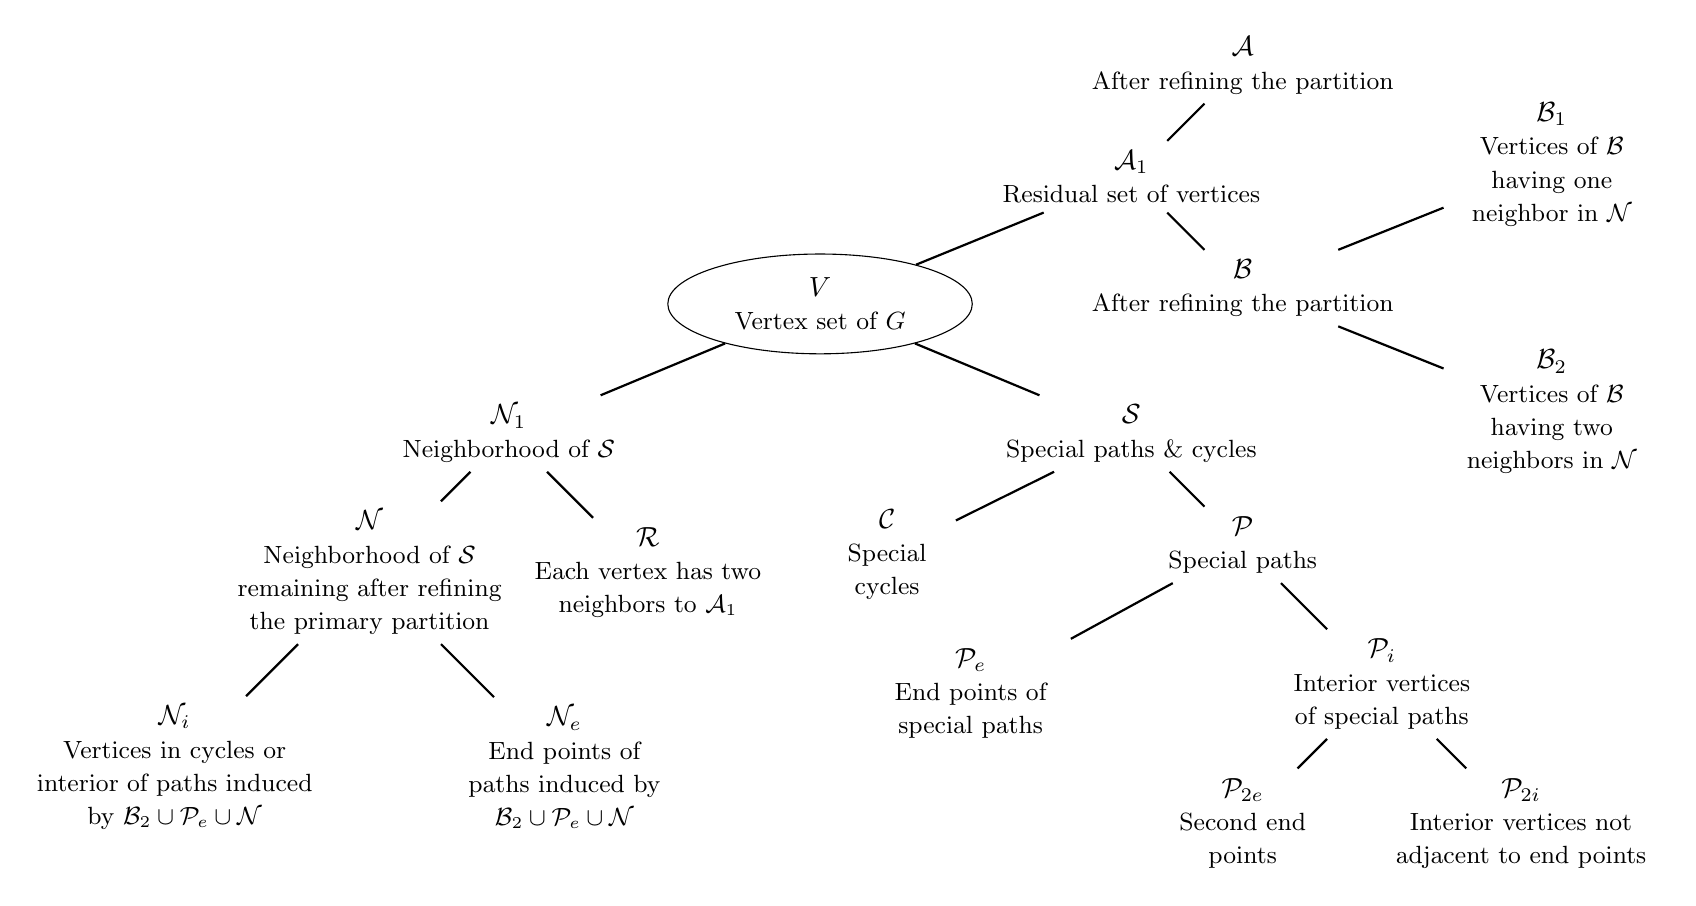
\begin{tikzpicture}
[node distance=1cm]
%%
\node[ellipse,draw] (V) at (0,0) {\parbox[c]{2.5cm}{\centering{$V$\\ \small{Vertex set of $G$}}}};
%% special paths & cycles
\node[node distance=1cm,below right=of V] (S) {\parbox[c]{3.5cm}{\centering{$\mS$\\ \small{Special paths \& cycles}}}};
\node[node distance=.5cm,below left=of S] (C) {\parbox[c]{1.5cm}{\centering{$\mC$\\ \small{Special cycles}}}};
\node[node distance=2cm,below right of=S] (P) {\parbox[c]{2.5cm}{\centering{$\mP$\\ \small{Special paths}}}};
%
\node[node distance=1cm,below left=of P] (Pe) {\parbox[c]{2.5cm}{\centering{$\mP_e$\\ \small{End points of special paths}}}};
\node[node distance=2.5cm,below right of= P] (Pi) {\parbox[c]{2.5cm}{\centering{$\mP_i$\\ \small{Interior vertices of special paths}}}};
\node[node distance=2.5cm,below left of= Pi] (P2e) {\parbox[c]{2.5cm}{\centering{$\mP_{2e}$\\ \small{Second end points}}}};
\node[node distance=2.5cm,below right of= Pi] (P2i) {\parbox[c]{3.5cm}{\centering{$\mP_{2i}$\\ \small{Interior vertices not adjacent to end points}}}};
%% edges
\draw[thick] (V) -- (S) -- (C);
\draw[thick] (S) -- (P) -- (Pe);
\draw[thick] (P) -- (Pi) -- (P2i);
\draw[thick] (Pi) -- (P2e);
%
%% neighbors
\node[node distance=1cm,below left=of V] (N1) {\parbox[c]{3.5cm}{\centering{$\mN_1$\\ \small{Neighborhood of $\mS$}}}};
\node[node distance=2.5cm,below left of=N1] (N)
{\parbox[c]{3.5cm}{\centering{$\mN$\\ \small{Neighborhood of $\mS$
remaining after refining the primary partition}}}};
\node[node distance=2.5cm,below right of= N1] (R)
{\parbox[c]{3.5cm}{\centering{$\mR$\\ \small{Each vertex has two neighbors
to $\mA_1$}}}};
\node[node distance=3.5cm,below right of=  N] (Ne) {\parbox[c]{2.5cm}{\centering{$\mN_e$\\ \small{End points of paths induced by $\mB_2\cup\mP_e\cup\mN$}}}};
\node[node distance=3.5cm,below left of= N] (Ni) {\parbox[c]{3.5cm}{\centering{$\mN_i$\\ \small{Vertices in cycles or interior of paths induced by $\mB_2\cup\mP_e\cup\mN$}}}};
%% edges
\draw[thick] (V) -- (N1) -- (N) -- (Ne);
\draw[thick] (N1) -- (R);
\draw[thick] (N) -- (Ni);
%% residual
\node[node distance=1cm,above right=of V] (A1) {\parbox[c]{3.5cm}{\centering{$\mA_1$\\ \small{Residual set of vertices}}}};
\node[node distance=2cm,above right of= A1] (A)
{\parbox[c]{4.5cm}{\centering{$\mA$ \\{\small After refining the partition}}}};
\node[node distance=2cm,below right of= A1] (B)
{\parbox[c]{4.5cm}{\centering{$\mB$\\{\small After refining the partition}}}};
\node[node distance=.25cm,above right =of B] (B1)
{\parbox[c]{2.5cm}{\centering{$\mB_1$\\ \small{Vertices of $\mB$ having one
neighbor in $\mN$}}}};
\node[node distance=.25cm,below right =of B] (B2)
{\parbox[c]{2.5cm}{\centering{$\mB_2$\\ \small{Vertices of $\mB$ having two
neighbors in $\mN$}}}};
%% edges
\draw[thick] (V) -- (A1) -- (A);
\draw[thick] (A1) -- (B) -- (B1);
\draw[thick] (B) -- (B2);
\end{tikzpicture}
{}
\end{document}
